\documentclass[10pt,journal,compsoc]{IEEEtran}
\usepackage{amsmath}
\hyphenation{op-tical net-works semi-conduc-tor}
\usepackage{graphicx}

\begin{document}
\begin{titlepage}
	\centering
	{\scshape 6.033: Computer Systems Engineering  \par}
	\vspace{3cm}
	{\scshape\LARGE Massachusetts Institute of Technology \par}
	\vspace{1cm}
	{\scshape\Large Final Design Project \par}
	\vspace{1.5cm}
	{\huge\bfseries Flux Vector Network Optimization\par}
	\vspace{2cm}
	{\Large\itshape Kenneth Friedman\par}
		{\Large\itshape Joel Gustafson \par}
			{\Large\itshape Obasi Onuoha \par}
	\vspace{.25cm}
	\textit{{\small\{ksf,joelg,ojonuoha\}@mit.edu}}
	\vfill
	Recitation Instructor\par
	Asaf Cohen. R12, R14

	\vfill

	{\large May 4, 2016\par}
\end{titlepage}

		
	% The paper headers
	\markboth{6.033: Computer Systems Engineering, MIT, Spring 2016}{}
	
	\IEEEtitleabstractindextext{%
		\begin{abstract}
			Improving the performance of the wireless network is of obvious interest to MIT. The task is to implement a system which optimizes the connections between clients and the MIT wireless network in order to improve the overall performance of the network. This paper proposes such a system.\\
			\\
			The design revolves around three modules: each client will have a \emph{controller} which communicates its requirements to an \emph{access point} which collects data about the traffics and clients to send to the \emph{server}. The \emph{server} ingests data about the network, stores it, and distributes connection instructions to the rest of the network.
		\end{abstract}}
			
		% make the title area
		
		%\titlepage
		
		\section{High Level System Overview}
		MIT is a large, highly institution; as such, it requires a robust wireless networking system.  This paper responds to the RFP sent out by the 6.033 course staff. As such it addresses  the specific requirements therein; the proposed system will connect all clients to a nearby AP with acceptable performance levels, it will allow for high network utilization even under periods of heavy load, and it will collect network usage data to aid MIT IS\&T in network management.\\
		\\
		Beyond the requirements established in the RFP, the proposed system adheres to three primary design goals: simplicity, scalability, and performance. There are many devices involved in the MIT wireless network and there are many people tasked to manage them. Consequently, the proposed system strives for simplicity to allay management difficulties and ease implementation. To that end, the majority of computation and decision making is relegated to the server module. This means that most updates will only have to take place in one location. It also means that any server side optimization model which complies with the proposed communication standards could be slotted into the system with very little, if any, changes to the remaining network infrastructure.\\
		\\
		Next, focus was placed on the twin goals of scalability and performance. MIT continues to grow in both human and geographic size. Consequently, the proposed system needs to be robust against changes in both the shape of the network and the number of users. Additionally, MIT hosts many events which radically increase the number of users to a relatively small portions of the network; the proposed system needs to handle local user spikes very well. This dovetails with performance, as all of these additional users will expect reasonable levels of speed and connectivity.
		
		\subsection{System Modules}
		The system contains three modules. The first module is the client, which is any device that wants to wirelessly connect to MIT's network. Each client has a controller, which contains information about the requirements of the given client. The second type of module is the access point, or AP. APs are located throughout MIT's campus, and they contain client information and provide network access. Finally, the third module is the server. The server is the central component that stores information and issues instructions.
		
		\subsection{Module Interaction}
		There is a straightforward interaction model between the three modules. Clients communicate information to APs. APs synthesize information from clients, and send that data to the server. The server then processes the incoming information and sends instructions to APs about which clients need to switch APs. The server also logs the network state for analytic purposes. This overview can be seen in Figure \ref{fig:overview}. 
		
        \begin{figure}
            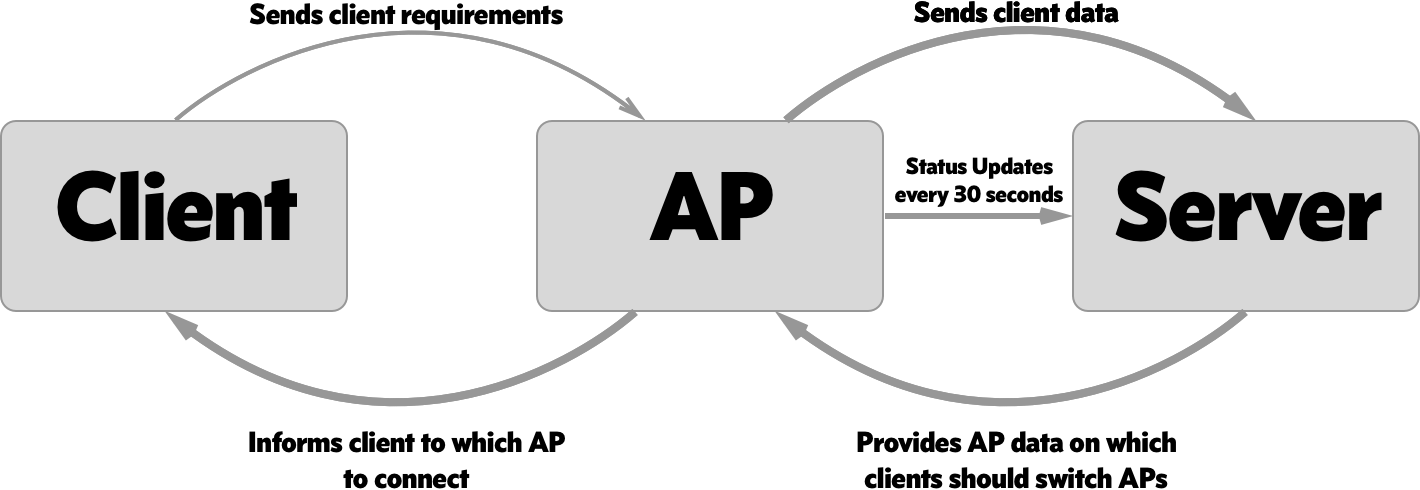
\includegraphics[width=\linewidth]{overviewDiagram.png}
            \caption{High Level Module Interaction Overview}
            \label{fig:overview}
        \end{figure}
		
		
		\section{Client}
		In order to preserve our goal of simplicity, the client performs little work with regards to the overall network. Each client contains a monitor and a controller. The monitor records the performance of the application running on the client. The controller takes the monitor's data and prepares it for transmission to the AP. The details of the communication are described in detail in section 5.1.\\
		\\
		No device is born connected to a network; it must discover them itself. The controller begins the connection and communication process by repeatedly cycling through all eleven 802.033 channels, listening for AP heartbeats for 40 milliseconds each. When the client receives a heartbeat, it will log its signal strength and the respective AP’s address, but continue searching for one more complete cycle, logging the signal strengths and addresses of any other APs it detects. After completing the extra victory lap, the client will select from its log the AP with the strongest signal strength, and selects it for initial connection.
		
		\section{Access Points}
		Networks can have tens of thousands of access points (APs), and may install, move, or remove them frequently. In order to keep all the access points easily maintainable, the proposed system design uses AP primarily as thin clients to forward data and requests to and from the central server and the client, simplifying the design and minimizing AP logic. This section provides a high-level overview of the functions of each AP beyond serving client requests for data from the outside internet, while section 5 describes the technical specifications for communication between network devices.
		
		\subsection{Client Connection}
		When a client connects to an AP, the AP forwards the client's initial connection message to the server, as detailed in sections 5.1 and 5.3. At this point, both the AP and the client assume that the client will remain connected to the AP unless explicitly reassigned by the server - a response is not needed or expected. This both reduces the number of messages and preserves a moderately functional network in event of a server failure.
		
		\subsection{Client Reassignment} Upon receiving a client reassignment message, an AP will forward it to the appropriate client, if it exists. The AP assumes no responsibility for ensuring that the client disconnects, and will continue serving its requests in the interim. The format of these messages are detailed in sections 5.2 and 5.4.
		
		\subsection{Network Statistics}
		Clients send their updated network demands and performance statistics to their AP at 30-second intervals. The AP aggregates these numbers and relays them to the server every 30 seconds. However, since clients operate independently of each other, each AP maintains a hash table mapping its clients' MAC addresses to their 64-bit \textit{data} integers from the update messages detailed in section 5.1. When an AP receives an update message from a client, it writes the value in the hash table at the client's MAC address key to be the 3-tuple \((G, A, T_S\)), where \(G\) is 32-bit integer from the first half of \textit{data}, \(A\) is the 32-bit integer from the second half of \textit{data}, and the timestamp \(T_S\) is the current time in seconds (only the seconds - 4 bits - are necessary, although this is an implementation detail). When the AP needs to send  update message to the server, it first computes \(G_S\) and \(A_S\), which are the sum of \(G\) and \(A\), respectively, for every value in the AP's hash table whose timestamp \(T_S\) is less than 35 seconds old. If a \(T_S\) is older than 35 seconds, the corresponding key is deleted from the table and the client is assumed to be disconnected. The AP then sends \(G_S\) and \(A_S\) to the server, as described in section 5.3.
		
		\section{Server}
		The majority of the computational complexity is handled by a central server, connected via reliable wired connection to all APs, which aggregates network data and manages client reassignment. The server is explicitly designed to be both unnecessary and modular: the network will still function, albeit naively, upon server failure, and the specific algorithms used to determine client reassignment are independent of the rest of the system. In this context, the server can be viewed as an aggressive optimization layer on top of the main network infrastructure that computes a relative local load factor for each AP and dispatches client reassignment messages to balance this accordingly. \\
		\\
		This dovetails well with the design goals of simplicity and performance. From a simplicity standpoint, a system such as this is much easier to design, deploy, and maintain. Additionally, it reduces potential error sources significantly. With regards to performance, designing the server as an optimization layer removes it as a point of failure. A system designed in this manner does not have a single point of failure, effectively guaranteeing some performance even under the most adverse conditions.\\
		\\
		This section details the components of the central server and their interactions with the rest of the system.
		
		\subsection{Network State Object}
		The server maintains network state in a custom data structure that is both a hash table and an undirected graph. There is one node for each AP, which must be manually created or deleted when APs are added or removed. The hash table is indexed by AP MAC addresses, which map to objects that are the nodes of the undirected network graph. These objects store both static and dynamic properties of the corresponding AP:
		\begin{itemize}
			\item Precise location
			\item Generated transmission bits
			\item Successful transmission bits
			\item Number of connected clients
			\item Links to nodes of overlapping APs
			\item Load Factor
			\item Flux Vector
		\end{itemize}
		The client count and transmission bit numbers are from the most recent AP update message, and so are never out-of-date by more than 30 seconds. Each nodes also store an association list of references to the nodes of APs whose signal coverage overlaps with its position, which can either be precomputed using geolocation and signal range data, or dynamically updated using client range information received from AP messages. Load Factor and Flux Vector are described in sections 4.2.1 and 4.2.2, respectively.
		
		\subsection{Client Assignment}
		The primary role of the server is to dispatch client reassignment directives to balance load across APs. Perfect equilibrium will rarely be possible, since clients are restricted to connecting to APs within their range, so the algorithm must make a best attempt at balancing each local graph individually. However, the network is composed of a continuous mesh of APs, not discrete local graphs, so the algorithm must scale across the entire mesh as well. We implement relative local load balancing in three steps: computing a load factor for each AP, and computing the difference of load factors across each link, called ``flux vectors", and sending reassignment messages for flux vectors greater than a normalized capacity threshold. The following sections elaborate on each step of this process.
		
		\subsubsection{Load Factors}
		This is done by computing a load factor \(L\) for each AP with the following equation:
		\[L = G + (G-A)^2\]
		where \(G\) is the number of generated bits and \(A\) is the number of successfully transmitted bits in the last AP update. This relation was chosen as the load factor to give extra weight to information overflow, when the AP becomes the communication bottleneck for the client. Load factors are updated continuously on each AP status message.
		
		\subsubsection{Flux Vectors}
		A flux vector from one AP to another is defined as the difference between their load factors, such that the AP with the larger load factor will have a positive flux vector, and the AP with the lower load factor will have a negative flux vector.
		\[V_{AB} = L_A - L_B\]
		Every 15 seconds, the server iterates over every node, and sums the flux vectors for every link in the node's list of overlapping APs, then normalizes this value over the number of clients connected to the AP. 
		
		\subsubsection{Reassignment}
		If the resultant normalized value is over a global threshold \(T\), to be defined and tuned by the network administrator, the server will direct the AP to reassign a proportional number of clients to the corresponding neighboring APs.
		
		\subsection{Network Analytics}
		In addition to client assignment routing, the server logs a snapshot of network traffic on each AP every second for IS\&T records. Although each individual AP only updates the server every 30 seconds to keep traffic on the server minimized, a second-by-second snapshot of every AP captures the state and load of the whole network with reasonable resolution.
		
		\section{Communications Protocols}
		This section outlines the communications protocols used from the controller of a client to the AP, from the AP to the controller of a client, from the AP to the server, and from the server to the AP.
		
		\subsection{Client to AP}
		When a client connects to an AP, its controller immediately sends a frame to the AP. The frame is of the following form:
		\begin{center}\textit{ src addr \textbar dst addr \textbar meta \textbar data  }\end{center}
		Where \textit{src addr} is the 48-bit MAC address of the client, \textit{dst addr} is the 48-bit MAC address of the AP to which the controller is communicating, and \textit{meta} is the 8-bit value 00000001. \textit{Data} is a variable-bit value defined as follows:
		\begin{center}\textit{R \textbar addrs}\end{center}
		Where \textit{R} is a 32-bit integer representing the maximum number of bits that the client will need to transmit over the course of any one second and \textit{addrs} is the value formed of the concatenation of the 48-bit MAC addresses of all of the APs within range of the client. The MAC addresses which compose \textit{addrs} are sorted in decreasing order of signal strength.\\
		\\
		Every 30 seconds, the client sends a message to its AP. This message is of the following form:
		\begin{center}\textit{ src addr \textbar dst addr \textbar meta \textbar data  }\end{center}
		Where \textit{src addr} is the 48-bit MAC address of the client, \textit{dst addr} is the 48-bit MAC address of the AP to which the controller is communicating, and \textit{meta} is the 8-bit value 00000100. \textit{Data} is a variable-bit value defined as follows:
		\begin{center}\textit{G \textbar A}\end{center}
		Where \textit{G} is a 32-bit integer representing the number of bits that the client generated over the past 30 seconds and \textit{A} is a 32-bit integer representing the number of bits that the client successfully sent over the past 30 seconds.
		
		\subsection{AP to Client}
		When an AP needs to tell a client to connect to a different AP within range of the client, it sends a frame of the following form:
		\begin{center}\textit{ src addr \textbar dst addr \textbar meta \textbar data  }\end{center}
		Where \textit{src addr} is the 48-bit MAC address of the AP sending the frame, \textit{dst addr} is the 48-bit MAC address of the client to which the AP wished to communicate, and \textit{meta} is the 8-bit value 00000010. \textit{Data} is 48-bit value specifying the AP to which the client should connect.\\
		\\
		When an AP needs to tell the user of a client to move physically in order to connect to a different AP which is not in the immediate range of the client, it sends a frame of the following form:
		\begin{center}\textit{ src addr \textbar dst addr \textbar meta \textbar data  }\end{center}
		Where \textit{src addr} is the 48-bit MAC address of the AP sending the frame, \textit{dst addr} is the 48-bit MAC address of the client to which the AP wished to communicate, and \textit{meta} is the 8-bit value 00000011. \textit{Data} is a 24-bit value defined as follows:
		\begin{center}\textit{bld \textbar rm}\end{center}
		Where \textit{bld} is a 12-bit binary integer specifying the building number of the desired AP and \textit{rm} is a 12-bit integer specifying the room number of the desired AP.
		
		\subsection{AP to Server}
		When a new client connects to an AP, it sends a message to the IS\&T server. This message is of the following form:
		\begin{center}\textit{maddr \textbar caddr \textbar R}\end{center}
		Where \textit{maddr} is the 48-bit MAC address of the AP, \textit{cddr} is the 48-bit MAC address of the client which just connected, and \textit{R} is a 32-bit integer specifying the maximum number of bits that the client will need to transmit over the course of any one second.\\
		\\
		Every 30 seconds, independent of any connected clients, the AP sends a message to the IS\&T server. This message is of the following form:
		\begin{center}\textit{maddr \textbar cnum \textbar rsum \textbar asum \textbar gsum}\end{center}
		Where \textit{maddr} is the 48-bit MAC address of the AP sending the message, \textit{cnum} is a 7-bit integer specifying number of clients connected to the AP sending the message, \textit{rsum} is a 39-bit integer specifying the maximum number of bits that the clients connected to the AP sending the message may need to send over any given second, \textit{asum} is a 20-bit integer specifying how many bits clients have transmitted to the AP sending the message over the last 30 seconds, and \textit{gsum} is a 39-bit integer specifying the number of bits that the clients connected to the AP sending the message have generated over the past 30 seconds. 
		
		\subsection{Server to AP}
		When the IS\&T server determines that an a client needs to connect to a different AP, it sends a message to the AP that client is currently connected to. This message takes the following form:
		\begin{center}\textit{caddr \textbar naddr \textbar rlct }\end{center}
		Where \textit{caddr} is the 48-bit MAC address of the client which is being directed to switch to a new AP and \textit{naddr} is the 48-bit MAC address of the AP to which the client is being directed to switch. \textit{rlct} is a 24-bit value composed of all 0's if the AP in question is in range of the client in question or a 24-bit value defined as follows if it is not:
		\begin{center}\textit{bld \textbar rm}\end{center}
		Where \textit{bld} is a 12-bit binary integer specifying the building number of the desired AP and \textit{rm} is a 12-bit integer specifying the room number of the desired AP.
		
		\section{evaluation}
		One of the most critical aspects of system design is evaluation. We will analyze the system and determine how well it achieves the design goals of simplicity, scalability, and performance. Additionally, we will evaluate the system against several metrics including communications overhead, various latencies, network utilization, and user happiness.
		
		\subsection{Communications Overhead}
		With consideration to our design goal of simplicity, the system attempts to send as few messages as possible. This also assists with our goals of scalability and performance, as fewer messages means less strain on the network.\\
		\\
		System messages from the Client to the AP and from the AP to the client are both small and infrequent. The Client's sends an initial connection message to the AP exactly once per connection and the AP sends a reconnect message to the client at most once per connection. Additionally, the Client sends the AP a status message once every 30 seconds. None of these messages are larger than 21 bytes. Even if an AP is at maximum capacity with 128 Clients, these communications use only a trivial fraction of an AP's bandwidth.\\
		\\
		Every AP sends the IS\&T Server one message per client per connection. Additionally, every AP sends the server one status message every 30 seconds. None of these messages is larger than 16 bytes. The server sends at most one message to an AP per client per connection. These messages are 11 bytes. In the worst case, this uses less than one thousandth of a percent of the 1Gbps connection between an AP and the server.
		
		\subsection{Usage Statistic Latency}
		Every 30 seconds, each AP sends the required usage statistics to the IS\&T server. The storing an exporting of these statistics is left to the server. Consequently, the server's model of the network state and usage is at most 30 seconds out of date. This means that IS\&T possess any usage data 30 seconds after it is collected.
		
		
		\section{Conclusion}
		We have presented this proposal in order to improve the quality of the MIT wireless network. We designed the system to be extremely scalable.  Utilizing a neural net allows the system to constantly update its assignment priorities as the network and its needs grow and change. Additionally, the adoption of this architecture realizes a very high performance system. Constant and consistent optimization ensures that desirable outcomes will be regularly attained. Finally, the proposed system places the primary load of computation on the server. This greatly simplifies the system and means that the majority of changes will not need to be propagated through the network.
		
		\section{Acknowledgments}
		The authors would like to thank Dr. Asaf Cohen, Jared Berezin, and Anubahv Jain for helpful discussions and useful feedback.
		
\end{document}